\documentclass[journal]{IEEEtran}

\usepackage{mathtools}
\usepackage{amsmath}
\usepackage{amssymb}
\usepackage{graphicx}
\usepackage{epstopdf}
\usepackage{cite}
\usepackage{array}
\usepackage{eurosym}
\usepackage{balance}
\usepackage{url}
\usepackage{verbatim}
\usepackage{color}
\usepackage{verbatim}

\newcommand{\hilight}[1]{\colorbox{yellow}{#1}}


\newcommand{\highlight}[1]{%
  \colorbox{yellow}{$\displaystyle#1$}}

\hyphenation{op-tical net-works semi-conduc-tor mo-nitoring}
\newcommand\blfootnote[1]{%
  \begingroup
  \renewcommand\thefootnote{}\footnote{#1}%
  \addtocounter{footnote}{-1}%
  \endgroup
}


\begin{document}

\title{4-PAM Modulation of Ambient FM Backscattering for Spectrally Efficient Low Power Applications} 
\author{
\IEEEauthorblockN{Spyridon Nektarios Daskalakis,~\IEEEmembership{Student Member,~IEEE}, Ricardo Correia,~\IEEEmembership{Student Member,~IEEE},
George Goussetis,~\IEEEmembership{Senior Member,~IEEE},
Manos M. Tentzeris,~\IEEEmembership{Fellow,~IEEE}, Nuno Borges Carvalho~\IEEEmembership{Fellow,~IEEE}  and 
Apostolos Georgiadis,~\IEEEmembership{Senior Member,~IEEE}
}

%\vspace{-1cm}
\thanks{
Manuscript received Month DD, YYYY; revised Month DD, YYYY; accepted Month DD, YYYY.
This work was supported 
by Lloyd's Register Foundation (LRF) and the International Consortium in Nanotechnology (ICON).
%
The work of M. M. Tentzeris was supported by the National Science Foundation (NSF) and the Defense Threat Reduction Agency (DTRA).
%
This work of  R. Correia and N. B. Carvalho was supported by the European Regional Development Fund (FEDER), through the Competitiveness and Internationalization Operational Programme (COMPETE 2020) of the Portugal 2020 framework, Project, MOBIWISE, POCI-01-0145-FEDER-016426 and is funded by FCT/MEC through national funds and when applicable co-funded by FEDER – PT2020 partnership agreement under the project UID/EEA/50008/2013.

This paper is an expanded version from the 2018 International Microwave Symposium (IMS) 2018, Philadelphia, Pennsylvania, USA, 10-15 June 2018.

S. N. Daskalakis, G. Goussetis and A. Georgiadis  are with School of Engineering \& Physical Sciences;  Institute of Sensors, Signals and Systems, Heriot-Watt University, Edinburgh, EH14 4AS, Scotland,
UK (e-mail: sd70@hw.ac.uk, g.goussetis@hw.ac.uk, apostolos.georgiadis@ieee.org).

M. M. Tentzeris is with School of Electrical and Computer Engineering, Georgia Institute of Technology, Atlanta, GA 30332-250, USA (e-mail: etentze@ece.gatech.edu).

R. Correia and  N. B. Carvalho  are with  
Departamento de Electr\'{o}nica, Telecomunica\c{c}\={o}es e Informática, Instituto de Telecomunica\c{c}\={o}es, Universidade de Aveiro,
3810-193 Aveiro, Portugal (e-mail: rjoao@ua.pt, nbcarvalho@ua.pt).
}}


%
\maketitle

\begin{abstract}
%

Ambient backscatter uses radio frequency signals available in the environment (e.g. radio broadcasting, television or mobile telephony) to transmit data effectively leading to significant  energy and cost efficiency increase. 
%
This paper presents a novel wireless tag, which for the first time utilizes  $4$-pulse amplitude modulation ($4$-PAM) technique
to modulate the  ambient  backscattered   FM signals
in order to send data to a nearby low-cost software defined radio reader.
%
The tag is based on an RF front-end that uses a single transistor controlled by an ultra low-power microcontroller.
%
The microcontroller includes an analog-to-digital converter (ADC) for sensing and a digital-to-analog converter (DAC) for RF front-end control.  
%
A proof-of-concept prototype is demonstrated in an indoor environment with the low bit rate of  $345$~bps and  power consumption $27~\mu$W. 
%
It operated using a real FM station at $34.5$~Km away and the tag-to-reader distance was tested at $1$~m.
%
The value of energy spent in this modulator was $78.2$~nJ/bit at $345$~bps and $27.7$~nJ/bit at $10.2$~Kbps.
% Spiro - I have not read the full paper but I suspect when you define the range this should also be associated with a given data rate and a quality of service (e.g. BER)
%

\end{abstract}
\begin{IEEEkeywords}
Ambient backscattering, backscatter communication, FM modulation, Internet-of-Things (IoT), Pulse Amplitude Modulation (PAM), radio frequency  identification (RFID) sensors, software-defined radio (SDR). 
\end{IEEEkeywords}




\IEEEpeerreviewmaketitle



\section{Introduction}
%
%
\IEEEPARstart{O}{ne} of the key challenges for  practical Internet-of-Things (IoT) and wireless sensor networks is the delivering autonomy to a massive number of devices which conventionally need to be powered with batteries. 
%
Moreover, ensuring low cost is an equally important  parameter pertaining to the viability of such systems.
%
Low-power and low-complexity backscatter communications have emerged as a promising paradigm to address aforementioned challenges. 
%
This technology delivers ultra-low-cost and ultra-low-power wireless communications by modulating the reflection of  incident radio frequency (RF) carrier signals.
%
Due to their advantageous features, backscattering communications
have been increasingly exploited in radio frequency identification (RFID) systems \cite{EPCRFID}.

In order to maintain low-cost and power efficient operation, the RF topologies of typical sensor nodes (tags) preferentially involve an antenna and a circuit with a single RF transistor, as for example in \cite{daskalakis2014soil}. 
%
The communication setup can be implemented in a bistatic or monostatic architecture  and requires an RF carrier wave (CW) emitter, the tag  and a reader.  
%
Traditional batteryless RFID systems utilize monostatic architectures were the reader includes the transmitter (CW emitter) and the receiver.
% 
Binary  amplitude shift keying or phase shift keying (ASK or PSK) modulations are commonly used for the communication between the tag and reader, such that information is encoded using two states of the amplitude or the phase of the reflected CW \cite{daskalakis2018uw}.
%
For example in the WISP platform \cite{sample2008design}, the electronic product code (EPC) protocol employs 2-ASK modulation to encode the  bits \texttt{1} and \texttt{0}  with long and short gaps in RF power, respectively.
%
Recently,  a body  implanted device  powered by a $13.56$~MHz wireless power transfer (WPT) link,  uplinks neural  data at $915$~MHz using a binary (BPSK) backscatter modulation \cite{kampianakis2017dual}.
%
In the aforementioned examples, the reader provides the CW  for supply and communication purposes. 


In order to increase the data rate, other works have exploited higher order modulation schemes for semi-passive and passive sensor networks \cite{thomas2010qam,thomas2012quadrature, kimionis2017millimeter}. 
%
In \cite{thomas2012quadrature} the authors present a $4$-quadrature amplitude modulation (QAM) scheme for backscatter communication enabling the transmission of $2$~bits per symbol instead of $1$~bit  with $2$-ASK, effectively increasing the data rate and leading to a reduced on-chip power consumption.
%
The modulator involved a battery-assisted (semi-passive)  and a passive tag operating in the range of  $850-950$~MHz.
%
This system demonstrated transmission of $4$-PSK/$4$-QAM   with  a bit rate  of $400$~kbps and with  static power dissipation of $115$~nW.
%
The backscatter modulator uses four lumped impedances  connected to an RF switch and it  was controlled by a microcontroller. 
% 
The same authors developed a $16$-QAM modulator for ultra high frequency (UHF) backscatter communication with five switches. 
%
Using a $16$-to-$1$ multiplexer, they were able to modulate the antenna load  between $16$ different states \cite{thomas201296}.
%
The tag was tested on  a $915$~MHz, $+23$~dBm,  CW signal.
% 
The tag-to-reader range was measured at $1.24$~m with a high bit rate $96$~Mbps. 
%
In \cite{correia2017quadrature} a novel backscatter modulator is presented which employs a Wilkinson power divider and two switches. 
%
The  divider introduces a phase shift  in one of the branches and two transistors acting as switches.
%
High order backscatter modulations  of M-QAM or M-PAM  can be achieved as each transistor can be controlled with different voltage levels to achieve different reflection coefficient values.   
%
The  $16$-QAM modulator demonstrated in \cite{correia2017quadrature}
features an   energy consumption as low as $6.7$~pJ/bit for a bit rate of $120$~Mbps.
%
 Reference \cite{shirane201513} presents a $5.8$~GHz RF-powered Si CMOS transceiver   with $32$-QAM communication scheme.
%
The uplink part uses the  backscattering technique   with a modulation $32$-QAM while consuming $113~\mu$W at $0.6$V. 
%
The RF font-end of the design consists of two transistors and the quadrature modulation is realized by two  intermediate frequency (IF) signals (I/Q).
%
In \cite{boyer2014invited}  a tutorial survey of backscatter modulation is  provided as an emerging means for short-range low-rate communications.
%
It provides the  relationship between on-tag
power harvesting and forward error correction applied to the higher order modulation  work \cite{thomas2010qam}.
%


\begin{figure}[t]
\centering
\includegraphics[width=0.85\columnwidth]{Figures/Fig1.eps}
\caption{FM ambient backscatter communication scheme. An example application  could be the identification of clothes in a mall using tablets and low cost SDRs.}
\label{fig:consept}
\end{figure}
%
In recent works,   existing ambient RF signals  have been proposed for backscatter communication instead of a CW emitter signal  \cite{liu2013ambient, van2017ambient}. This approach simplifies the complexity and cost of the system and its deployment.
%
Reference \cite{liu2013ambient} presents two RF-power devices that communicate between them exploiting the scattering of ambient TV signals.
%
In  \cite{qian2018iot}, a backscatter PSK hardware prototype is presented that combines a $4$-PSK transmitter, an energy harvester and a multi-level voltage detector. 
%
Two similar prototypes can communicate  with data rate of $20$
kbps using an ambient signal from UHF TV band.
%
In \cite{correia2018dual} a dual-band 4-QAM backscatter modulator circuit was proposed for ambient signals. 
%
It is composed by two transistors and a dual-band Wilkinson power divider, following the same principle proposed in \cite{correia2017quadrature}.
%
The  modulator presents an average power consumption of
$27$~nW for $500$~kbps of data rate at $900$~MHz and
$2.45$~GHz (cellular and Wi-Fi frequencies).
%
In \cite{wang2017fm}, broadcast frequency modulated (FM) signals have been used to power the tag and  enable effective communication between tag and reader. 
%
The transmitted power of FM signals is higher than AM signals, TV and GSM signals and hence can deliver better communication range between the tag and reader.
%
The initial implementation of \cite{wang2017fm} was able to communicate over distances of several feet, even in cases where transmission towers were up to many kilometers away. 
%

Our previous work \cite{daskalakis2017ambient} demonstrated a tag  capable of transmitting FM reflections  to a computer or a tablet through a low-cost software defined radio (SDR) reader.
%
Fig.~\ref{fig:consept} depicts a possible application of this system. 
%
The tag uses ASK binary modulation with FM0 encoding on ambient FM station signals as in commercial RFID systems. 
%
The FM transmitter was $34.5$~Km away from the measurement's setup and a $5$~m communication range between the tag and the reader was achieved with $2.5$~Kbps bit rate. 
%
A theoretical analysis of the error rate performance  also provided \cite{daskalakis2017ambient}.
%


In \cite{wang2017fm} for the first time  high order modulation  was introduced for ambient backscattering communications. 
%
The authors demonstrated $4$ frequency-shift keying (FSK) modulation to transmit two bits per symbol over the ambient FM signals with a maximum data rate $3.2$~kbps.
%
The work involves simulation of an integrated circuit for the tag, while for the prototype an arbitrary waveform generator (AWG) was used connected with an RF front-end.


In this work we consider high order amplitude modulation 
and we demonstrate the first prototype suitable for ambient backscatter communication deployment working with $4$-PAM.
%
 The FM frequencies were selected due to the strong ambient signal source that can be used for backscatter communication.
%
The $4$-PAM  modulation is used to double the bit rate, compared to a $2$-PAM system.
%
With amplitude modulation the complexity of the  receiver and the tag can be drastically simplified as there is no need for a different frequency for each symbol.
%
Tag and receiver are more complex as variation of modulating signal has to be converted and detected from corresponding variation in frequencies.
%
Preliminary results were presented in previous work  \cite{daskalakisims2018}, where  $4$-PAM scheme was selected due the low hardware complexity and low power consumption.
%
This work is an extensive presentation of the 
FM backscatter system  in \cite{daskalakisims2018} thus theoretical analysis of the system is provided as well as a real time receiver implementation. 
%
Additional details about the tag are also provided. 
%
In particular, our tag employs a single low cost transistor and a telescopic antenna achieving communication with low bit rate for reduces power consumption.
%
This work differs from \cite{thomas201296, correia2017quadrature} since it uses ambient FM signals as the carrier instead of an intentionally transmitted unmodulated CW signal.
%
The use of FM signals on the receiver increases the complexity of selecting the thresholds associated with demodulation, as explained below in Section~\ref{Sec:receiver}.
%
In particular,  we present a  tag consisting of  a micro-controller (MCU) with a digital-to-analog converter (DAC)  and an analog-to-digital converter (ADC).
%
The tag could collect data from sensors through the ADC and process them. 
%
The MCU creates the modulation pulses internally and controls the RF front-end transistor via the DAC.
%
A low cost SDR receiver is used similarly to \cite{daskalakis2017ambient}.   
%


This paper is structured as follows: Section~\ref{Sec:back} reviews the  principles of the proposed backscatter communication systems. 
%
Section~\ref{Sec:tag} describes the tag hardware implementation. 
%
Section~\ref{Sec:PAM} provides the theory and performance
analysis of the FM ambient $4$-PAM  technique.
%
Section~\ref{Sec:receiver} discusses the theory, as well as the hardware and software elements of the receiver.
%
In Section~\ref{Sec:Experimental}, the proof-of-concept experimental communication  results are presented.
%
Section~\ref{Sec:Discussion} provides the comparison of our work with other similar high order modulation works.
%
Finally, section~\ref{Sec:Conclusion} concludes this work.



\section{Backscatter Modulation}
\label{Sec:back}
%
\begin{figure}[t]
\centering
\includegraphics[width=1\columnwidth]{Figures/Fig2.eps}
\caption{Backscatter radio principle: An RF transistor alternates the termination loads $Z_\text{i}$ of the antenna corresponding to different  reflection coefficients $\Gamma_\text{i}$. Four reflection coefficients ($n=4$) could create a four pulse amplitude modulation ($4$-PAM).}
\label{fig:backscatter}
\end{figure}
%
In backscatter communications, the tags do not need to transmit a radio signal, since they reflect signals transmitted by the reader or another ambient radio emitter.
%
A backscattering tag modulates the reflected signal using one or more transistors or RF switches connected to the antenna as it is shown in Fig.~\ref{fig:backscatter}.
%
A  binary backscatter communication is  based on a reflected waveform that should switch between a fully matched 
and a short circuit load terminating the antenna.
%
In previous work \cite{daskalakis2017ambient}, an RF switch  was directly connected to the RF front-end  antenna in order to create the two discrete states.
%
For high order  modulations, the number of states have to be increased and the RF circuit  must create a specific  discrete impedance for each transmitted symbol.
%
For this purpose, a single RF  transistor circuit can be used as an active load in order to create different impedances for the PAM constellation  \cite{correia2017quadrature}.
%
In this work an E-pHEMT transistor was used to implement a circuit compatible with a $4$-PAM scheme. 
%
The RF circuit presents four distinct impedance values for a four different gate voltages. 
%
A given antenna with impedance $Z_\text{a}$ connected to a complex load with impedance $Z_\text{i}  \in \lbrace Z_\text{1} ,Z_\text{2} , Z_\text{3} ,Z_\text{4}  \rbrace$, is associated with a reflection coefficient obtained as:
%
\begin{align}
\Gamma_\text{i}=\frac{Z_\text{i}-Z^{*}_\text{a}}{Z_\text{i}+Z_\text{a}}.
\label{eq:gamma}
\end{align}
%
Typically the antenna impedance is  chosen to be  $50$ Ohm. By changing the gate voltage of the transistor, four distinct reflection coefficients can be achieved corresponding to the four symbols. 
%
\begin{table}[t]	
\renewcommand{\arraystretch}{1}
\centering
\caption{$4$-PAM Modulation Parameters}
\scalebox{1}
{
\begin{tabular}{c|c|c|c}
\hline
\hline
%\begin{tabular}[x]{@{}c@{}}MSE(Hz$^2$)\\pre-filt.\end{tabular} For forcing newline in cell
 $\Gamma_\text{i}$& Symbol & Bits & $V_\text{gate}$ (mV) \\
\hline
\hline
 $-0.7245 - j0.6922$ &$-3$ & \texttt{00} &$0$ \\
\hline
 $-0.3414 - j0.2881$&$-1$ & \texttt{01} &  $333$\\
\hline
$+0.0223 + j0.1779$&$+1$ &\texttt{11}  &  $387$
    \\
\hline
$+0.3079 + j0.6334$&$+3$ &  \texttt{10} & $600$ \\
\hline
\end{tabular}
}
\label{tab:gammas}
\end{table}
%
The performance of PAM modulation is optimized when the $\Gamma_\text{i}$ values lie equidistantly along a straight line on the Smith Chart (Fig.~\ref{fig:backscatter}, left) \cite{correia2017quadrature}.
%
Considering the above, we can select the desired values of the reflection coefficients; an example of four equidistant measured values on the same line is shown in  Table~\ref{tab:gammas}.
%
Using this table and (\ref{eq:gamma}), the desired voltage values at the transistor gate can be obtained. 

\begin{figure}[t]
\centering
\includegraphics[width=0.7\columnwidth]{Figures/Fig3.eps}
\caption{Schematic  of Proof-of-concept tag. A low power micro-controller reads the sensors and controls the RF front-end circuit.}
\label{fig:shem_tag}
\end{figure}
%
%
%
The  received signal can be expressed in the following complex baseband form \cite{daskalakis2017ambient}:
%
%
\begin{align}
\label{eq:yr}
y_r(t)=\big[ \alpha_{\text{dc}}e^{j\phi_{\text{dc}}}+\alpha_{\text{mod}}e^{j\phi_{\text{mod}}}  
\Gamma_\text{i} (t-\tau)\big]e^{-j2\pi\Delta F t} +n(t)
\end{align}
%
with  $\alpha_{\text{dc}}, \alpha_{\text{mod}}  \in 
{\Bbb R} $  and $e^{j\phi_{\text{dc}}}, e^{j\phi_{\text{mod}}} \in  [0, 2\pi)$.
%
The term $\alpha_{\text{dc}}e^{j\phi_{\text{dc}}}$
defines the dc component associated with the transmitter broadcast baseband signal.
% 
The term  $\alpha_{\text{mod}}e^{j\phi_{\text{mod}}}$  describes the scaling and rotation of the modulated  part  of the received  tag signal.
%
This component depends on a number of factors, including the  transmitter signal power, the channel characteristics associated with the links between the  transmitter-to-tag and tag-to-reader and the backscattering efficiency of the tag.  
%
The term $\Delta F$ represents the carrier frequency offset (CFO) between the transmitter (FM station) and the reader.
%
The term $n(t)$ is the complex thermal Gaussian noise at the receiver and the time constant $\tau$  depends on the tag-to-reader channel propagation characteristics. 
%
The tag signal is  a  function of $\Gamma_\text{i}$ over time.




\section{Sensor Node/Tag Design}
\label{Sec:tag}
 %
\begin{figure}[t]
\centering
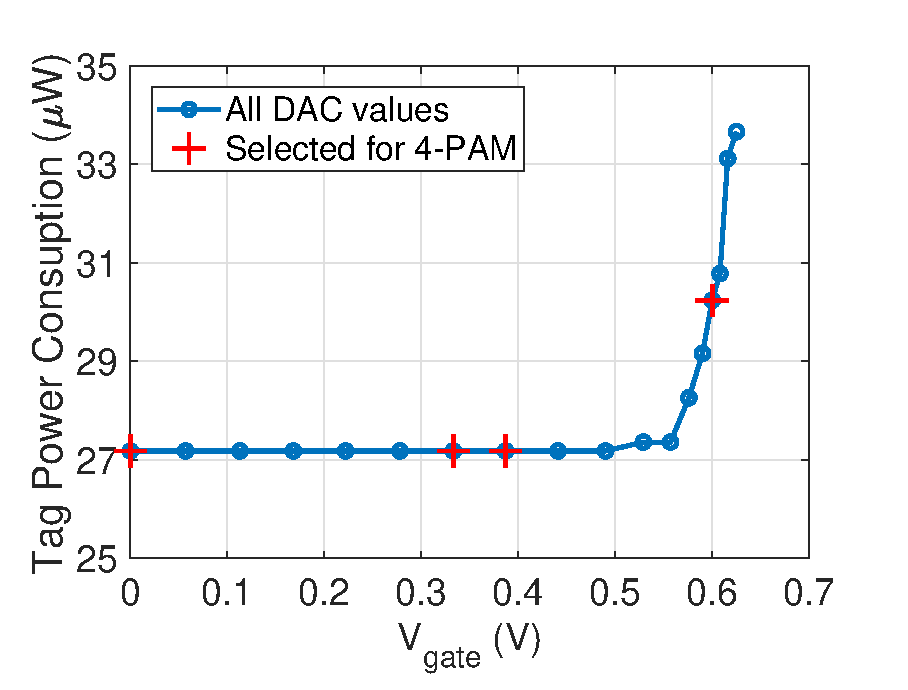
\includegraphics[width=0.8\columnwidth]{Figures/Fig4.eps}
\caption{Digital-to-Analog Converter   output voltage versus the tag power consumption. The tag was measured at $1.8$~V  when the ADC was turned off.
Four optimal  values were selected for the backscatter communication.}
\label{fig:dac_volts}
\end{figure}
%

%
Our tag consists of an  ultra low power MCU connected with an RF front-end as it is  depicted in the block diagram of Fig.~\ref{fig:shem_tag}.
%
The $8$-bit PIC16LF1459 MCU from Microchip Inc. was used, whitch   consumes $25~\mu$A/MHz of current at $1.8$~V \cite{PIC16LF1459}. 
%
The clock of the MCU was programmed at $32$~KHz in order to minimize the power consumption of the tag.  
%
The MCU also has a sleep mode operation with current consumption of $0.6~\mu$A.
%
The MCU includes a $10$~bit  ADC  and collects data from analog sensors on the tag. 
%
%
The $5$-bit DAC of the MCU is used in our application  to drive the RF front-end transistor with different voltages. 
%
The DAC has the ability to supply the gate of the transistor with  $32$
distinct voltage levels in order to change the antenna load impedance.
%
Fig.~\ref{fig:dac_volts} depicts the tag power consumption for all the possible 
DAC output voltages when the MCU was supplied by a $1.8$~V voltage source.
%
The figure shows the voltages up to $0.625$~V, since the maximum voltage for the transistor (DAC output), in our application was $0.6$~V.
%
Four DAC outputs were selected for our backscatter modulation scheme as it is explained in more details below.
%
The tag was powered by the flexible solar panel, SP3-37 provided
by PowerFilm Inc. \cite{SP3-37}.  
%
The solar panel charges a $220~\mu$F  tantalum capacitor instead of a battery through a low-voltage-drop Schottky diode.
%
An external voltage reference IC XC6504 \cite{XC6504}  was also used  to supply the tag with a stable voltage ($V_\text{ref}$) $1.8$~V.
%
The proposed sensor node does not focus on a specific  sensing application  or power management system but only on the novel telecommunication part of the system. 
%
An  RF harvester could be designed in the future \cite{assimonis2014efficient} to charge the capacitor during the night in combination with solar cell during the day \cite{niotaki2014solar}.
%
Another idea is an integrated cooperative harvester capable of collecting both electromagnetic 
and kinetic energy simultaneously as proposed in
\cite{gu2018integrated}.



The RF front-end consists of the ATF52189 E-pHEMT RF transistor from Broadcom \cite{ATF52189} and the SRH788 monopole antenna.
%
The maximization of the magnitude of  complex reflection coefficient
differences between the four states is a main objective  for optimized backscatter communication \cite{BleDimSah:j10}.
%
In this work, a core RF circuit challenge was to achieve the desired change of the drain impedance by varying the voltage at the gate in the range between $0$ to $0.6$~V. 
%
The Advanced Design System (ADS) from Keysight was used for the optimization of the RF front-end circuit. 
%
The simulations  performed involved the variation of the gate voltage at the transistor from $0$ to $0.6$~V with a sweep of $0.01$~V from $87.5$~MHz to $108$~MHz.
%
More specifically  the large-signal S-parameter simulation was used to perform the backscatter modulation in order to maximize the distance between the consecutive $\Gamma_i$ values.
%
Following the aforementioned optimization procedure, the matching network between the transistor and the antenna was composed by a capacitor and an inductor as depicted in the schematic of Fig.~\ref{fig:shem_tag}.
%
In the simulation  we assumed that we have a ideal $50$~Ohm antenna connected with our RF front-end and
the optimum  component values were found to be $68$~pF and $27$~nH. 
\begin{figure}[t]
\centering
\includegraphics[width=0.9\columnwidth]{Figures/Fig5.eps}
\caption{The fabricated tag prototype  with  the RF front-end  board. The tags is powered by a solar panel.}
\label{fig:fabricated}
\end{figure}


The RF front-end board was fabricated on Astra MT77 substrate with thickness $0.762$~mm, $\epsilon_r= 3.0$ and $tan\delta=0.0017$. 
%
%
The main  board of the proof-of-concept tag that integrates the MCU was fabricated on a Rogers RO4350B substrate.
%
The fabricated prototypes and the solar panel  are shown  in  Fig.~\ref{fig:fabricated}.
%
As mentioned, the output of the DAC was connected with the gate of the transistor on the RF front-end.
%
%
The fabricated  RF front-end board was measured using a vector network analyser (VNA) with $P_\text{in}=-20$~dBm at the frequencies of the FM band, $87.5-108$~MHz.
%
Each DAC output corresponds to a specific reflection coefficient $\Gamma_\text{i}$ and all the possible voltages of Fig.~\ref{fig:dac_volts} were tested through the VNA.
%
Four voltages: $0$, $333$, $387$ and $600$~mV were found as the optimum values to supply the gate of the transistor and create the $4$-PAM modulation.
%
The selected values are also depicted in Fig.~\ref{fig:dac_volts} creating  four impedances or symbols for a specific frequency.
%
The measured $\Gamma_\text{i}$  using the four voltages in the FM band are presented in Fig.~\ref{fig:smith}.
%
As it is observed, the selected voltage values offer almost equal distances between the corresponding $\Gamma_\text{i}$.
%
The prototype board was also tested at $-10$ and $-30$ dBm and were exported the same results with Fig.~\ref{fig:smith}. 
%
Table~\ref{tab:gammas} also shows  the resulting $\Gamma_\text{i}$ in combination with the symbols, the bits and the gate voltages at a fixed frequency of $95.8$~MHz.
%
Using the four voltages at the gate of the transistor and sweeping the frequency it is possible to observe that each state corresponds to an ``arc"  on the Smith Chart.
%
In particular, the set of  four states (each line in Fig.~\ref{fig:smith}) rotates clockwise as the frequency increases. 
% Spiro: Check what I wrote above and make sure it is correct, I am not sure what you meant
%
As per the design target, equal distances between the symbols were achieved assuming antenna input impedance equal with $50$~Ohms, in order to maximize the signal-to-noise ratio (SNR)  and thus the efficiency of the PAM modulation.
%
It is noted that our tag is a semi-passive design where the available capacitor  powers the  MCU during transmission from the tag to the reader. 
%
%According to \cite{nikitin2007differential},\cite{BleDimSah:j10} for semi-passive tags, the two pairs of symbols  and (-1 +1) must be diametrically opposite on two unit circles.
%(....how to explain more this?)
%I think this is alreadt addressed, no?
\begin{figure}[t]
\centering
\includegraphics[width=0.75\columnwidth]{Figures/Fig6.eps}
\caption{Smith Chart with measured reflection coefficient values for $4$ different voltage levels at the gate of transistor. 
The $Pin$ was fixed at $-20$~dBm for frequencies $87.5-108$~MHz.}
\label{fig:smith}
\end{figure}

\section{Ambient FM 4-PAM Modulation}
\label{Sec:PAM}
%

Pulse Amplitude Modulation (PAM) is a  method of sending information by scaling a pulse shape with the amplitude of the symbols and  duration $T_\text{symbol}$ \cite{johnson2011software}. 
% Spiro: add reference here. Better to take the definition from a book. I am not sure I can follow your definition above
In the $4$-PAM there are  four symbols and each symbol corresponds to  a pair of two bits.  
%
Each bit duration is denoted as $T_\text{bit}$ 
and the data bit rate is $2/T_\text{bit}$ bits per second (bps). 
%
According to $4$-PAM it is possible to transmit two bits with each symbol/pulse, for example, by associating the amplitudes of  \texttt{-3,−1,+1,+3}, with  four  bit choices \texttt{00}, \texttt{01}, \texttt{11}, and \texttt{10} (Table.~\ref{tab:gammas}).
%
\begin{figure}[t]
\centering
\includegraphics[width=0.7\columnwidth]{Figures/Fig8.eps}
\caption{The $4$-PAM symbols. Three thresholds are calculated for the decision.}
\label{fig:PAMsymbols}
\end{figure}
%
The symbols \texttt{$\pm$1,$\pm$3} are  shown in Fig.~\ref{fig:PAMsymbols} and the bit representation of the symbols is Gray coded \cite{proakis2008digital}. 
%
In order to transmit a digital stream, it must be converted into an analog signal. 
%
After conversion of the bits into symbols, the  analog form of a $4$-PAM modulation signal can be expressed as:
%
\begin{equation}
\Gamma_\text{i} (t-\tau) =\sum_{n=0}^{N-1} x_n \Pi[t- nT_\text{symbol} -\tau]
\label{eq:pulses_gamma}
\end{equation}
%
where $ x_n\in \lbrace -3,-1,+1,+3 \rbrace$, $N$ is the number of transmitted symbols and $\Pi(t)$ is a pulse with duration $T_\text{symbol}$.
%
Thus, each member of the $4$-PAM data sequence is multiplied by a pulse that is nonzero over the appropriate time window.



%
\begin{figure}[t]
\centering
\includegraphics[width=1\columnwidth]{Figures/Fig7.eps}
\caption{An oscilloscope measurement of the sending packet.  Voltage levels correspond to the $4$-PAM symbols at the gate of the transistor are presented.}
\label{fig:packet_tag}
\end{figure}

The proof-of-concept tag  was set up to send a fixed bitstream packet format. 
%
In this work the fixed  bit sequence was: \texttt{10001000100111-00-01-0111100011} which is translated to 
symbol sequence: \texttt{+3-3+3-3+3-1+1 -3 -1 -1+1+3-3+1}.
%
Transmission of some known
preamble data is required at the receiver to identify the beginning of a frame (packet) at the  transmission. 
%
Here the first seven symbols ($14$~bits) were added before the message sequence as a preamble.
%
The symbols of the preamble are used also  as training symbols as explained below.
%
After the preamble, ``Tag Number" bits ($2$~bits),  ``Sensor Number" bits ($2$~bits) and   ``Sensor Data" bits ($10$~bits) follow. 
%
The  ``Tag Number" bits  were utilized in case that four different  tags will be used in a future wireless sensor network.
%
With this allocation, the tag could support up to four sensors and  the ``Sensor ID" part is used to identify the sensor number.
% Spiro: is it not possible to add more bits here and hence allow for more tag IDs? If so please elaborate
The last $10$~bits section is used for transmitting the sensor data. 
%
An example of the  transmitted packet is depicted in Fig.~\ref{fig:packet_tag} and more bits could be added   in order to include extra sensors or tags.  
%


%
\section{Receiver}
\label{Sec:receiver}
\subsection{Receiver Theory}
%
FM radio stations typically operate in the range of frequencies from $88$~MHz to $108$~MHz and use frequency modulation in order to transmit the audio signals.
%
The FM  signals are described in \cite{daskalakis2017ambient}  and are given by the formulations $x_\text{FM}$  and $m(t)$ of the same work.
%
In our case, an FM modulated signal is used for communication instead of a CW signal and the complex baseband received signal is described by $y_\text{amp}(t)$ signal in \cite{daskalakis2017ambient} and  contains the rectangular pulses of  (\ref{eq:pulses_gamma}).

According  to \cite{daskalakis2017ambient} and \cite{qian2017noncoherent} we can simplify the  received complex signal as:
%
\begin{equation}
y_\text{amp}(t) \approx Ae^{-jD} e^{jK} h(t) + n(t)
\label{eq:y_t}
\end{equation}
%
with $h(t)= a_\text{1} (t)+a_\text{2}(t)b(t)$.  The term $D$ describes the frequency offset and the term $n(t)$ corresponds to the  white Gaussian noise added at the receiver with $n(t)\sim \mathbb{N}(0,N_\text{w})$. 
%
The term $h(t)$ contains  the useful data signal, $b(t)$, as well as the effects of the channels (FM station-to-reader, tag-to-reader).
%
In the above formulation we  assume that the tag and receiver are very close compared to the FM station distance so  $e^{jK}$ represents the common delay of the signal  received from the FM station. 
%
Initially, a  similar procedure as in \cite{daskalakis2017ambient}  is followed at the receiver. 
%
The received signal is $y_\text{amp}(t)$ and its envelope detector is taken in order to remove the CFO term.
% Spiro: what is CFO?
The obtained signal as in \cite{daskalakis2017ambient} is  
%
\begin{equation}
\begin{gathered}
Z(t) = A^{2} \vert h(t)\vert ^2 + w(t)
\end{gathered}
\label{eq:zt}
\end{equation}
with $w(t)$ Gaussian process\cite{qian2017noncoherent}:
 \begin{equation}
w(t)\sim \mathcal{N} \big(N_\text{w},N_\text{w}^2+2A^2 N_\text{w} \vert h(t)\vert ^2 \big).
\label{eq:w}
\end{equation}
%
The signal $Z(t)$ is correlated with a pulse $q(t)=1$ for $0< t\leq T_\text{symbol}$ and a synchronization procedure is then applied  in order to identify the stating point of the frame.
%
A dc removal is required for the synchronization; since the dc term  does not
contribute with any information on the transmitted data, it can be ignored in the remaining of the receiver processing.
%
The obtained signal can be expressed as:
\begin{equation}
\begin{gathered}
U_\text{i} =X_\text{i} +V_\text{i} = \\
\int_0^{T_\text{symbol}}  A^2  |h(t)|^2 q(t) \mathrm{d}t +\int_0^{T_\text{symbol}}  w(t) q(t) \mathrm{d}t.
\end{gathered}
\label{eq:zt}
\end{equation}
%
Using the $4$-PAM modulation, $|h(t)|^2$ can take four values ($h_i(t)$) with $ i\in \lbrace 1, 2, 3, 4 \rbrace$ and thus $V_\text{i}$ is a  Gaussian process:  
\begin{equation}
V_\text{i}\sim \mathbb{N} \left(T_\text{symbol}N_\text{w}, T_\text{symbol}^2 N_\text{w}^2+ 2T_\text{symbol}^2 A^2 N_\text{w} |h_\text{i}|^2  \right).
\label{eq:v}
\end{equation}
Using $X_\text{i} =T_\text{symbol}A^2 |h_\text{i}|^2 $ it is straightforward to show that $U_\text{i}$ is a Gaussian process
with $U_\text{i} \sim \mathbb{N} \left(\mu_\text{i}, \sigma_\text{i}^2 \right)$.
The  mean and variance are analysed as:
%
\begin{equation}
\mu_\text{i}= T_\text{symbol}A^2 |h_\text{i}|^2 +T_\text{symbol}N_\text{w},
\label{eq:m}
\end{equation}
%
\begin{equation}
\sigma_\text{i}^2= T_\text{symbol}^2 N_\text{w}^2+ 2T_\text{symbol}^2 A^2 N_\text{w} |h_\text{i}|^2. 
\label{eq:v}
\end{equation}
%
Our system works in  non-coherent mode 
where the algorithm  does not perform synchronisation between receiver and transmitter. 
%
A non-coherent algorithm does not use phase and frequency estimation techniques that add  complexity  and rate loss at the receiver  \cite{alevizos2016log}. 
%

For the symbol detection the minimum distance (Maximum-Likelihood) rule is used  thus no a priori information on the transmitted symbols is available for our system \cite{proakis2008digital}. 
%
The decision boundaries and the transmitted constellation  for a given measurement $U_\text{i}$, $ i\in \lbrace 0, 1, 2, 3  \rbrace$ are depicted in Fig.~\ref{fig:PAMsymbols}.
%
Three decision boundaries $t_\text{01}$, $t_\text{12}$ and $t_\text{23}$    are located between the
subsequent symbols.
%
They quantise the signal values as decisions are taken by comparing by comparing them with the thresholds.
%
If  the symbol error probability  can be defined as $P_\text{e}$ we can also evaluate the bit error probability (BER) as 
%
\begin{equation}
P_\text{b} =\frac{ P_\text{e}} {2}= \frac{1} {8} \sum_{i=0}^{3} P_\text{e,i}
\label{eq:pb}
\end{equation}
%
with $P_\text{e,i}$ the   error probability of each symbol.
%
For  example, when the symbol \texttt{-3} was sent,  the probability of error is the probability to decide in  the right side of threshold $t_\text{01}$ (Fig.~\ref{fig:PAMsymbols}) and it is defined as $P ( U>t_\text{01}|U_\text{0})$.
%
The conditional error probability for each symbol can be  calculated and simplified using Q-function  accordingly:
%
\begin{equation}
\begin{gathered}
P_\text{e0}= P ( U>t_\text{01}|U_\text{0})=Q \left(\frac{t_\text{01}-\mu_\text{0}} {\sigma_\text{0}} \right),\\
P_\text{e1}= P ( U>t_\text{12}|U_\text{1})+P ( U \leq t_\text{01}|U_\text{1})=\\
Q \left(\frac{t_\text{12}-\mu_\text{1}} {\sigma_\text{1}} \right)+Q \left(\frac{\mu_\text{1}-t_\text{01}} {\sigma_\text{1}}\right),\\
P_\text{e2}= P ( U>t_\text{23}|U_\text{2})+P ( U \leq t_\text{12}|U_\text{2})=\\
Q \left(\frac{t_\text{23}-\mu_\text{2}} {\sigma_\text{2}} \right)+Q \left(\frac{\mu_\text{2}-t_\text{12}} {\sigma_\text{2}}\right),\\
P_\text{e3}= P ( U\leq t_\text{23}|U_\text{3})=Q \left(\frac{\mu_\text{3}-t_\text{23}} {\sigma_\text{3}}\right)
\end{gathered}
\label{eq:qf}
\end{equation}
%
where 
$Q(x)= \frac{1} {\sqrt {2\pi}}\int_x^{\infty} e^{-t^2/2}\mathrm{d}t$  the $Q$ function.
%
For two adjacent conditional probabilities we can assume that:
\begin{equation}
P( U=t_\text{01}|U_\text{0})=P(U=t_\text{01}|U_\text{1})
\end{equation}
 which is expressed  as: 
\begin{equation}
\frac{1}{{\sigma_\text{0} \sqrt {2\pi}}} e^{-\left( {t_\text{01} - \mu_\text{0} } \right)^2 /2\sigma_\text{0}^2} = \frac{1}{{\sigma_\text{1} \sqrt {2\pi}}} e^{-\left( {t_\text{01} - \mu_\text{1} } \right)^2 /2\sigma_\text{1}^2}
\end{equation}
%
thus $U_\text{0}, U_\text{1}$ are Gaussian as it was mentioned before.
%
Using the above equality the threshold $t_\text{01}$ can be easily calculated as:
%
\begin{equation}
\begin{gathered}
t_\text{01} = \frac{\sigma_\text{1}^2 \mu_\text{0}-\sigma_\text{0}^2 \mu_\text{1}} {\sigma_\text{1}^2 - \sigma_\text{0}^2}\pm \frac{\sqrt{\sigma_\text{1}^2 \sigma_\text{0}^2 
\Big[(\mu_\text{1}-\mu_\text{0})^2 +(\sigma_\text{1}^2 - \sigma_\text{0}^2 )\ln \frac{\sigma_\text{1}^2}{\sigma_\text{0}^2}\Big] }} 
{\sigma_\text{1}^2 - \sigma_\text{0}^2}.\\
\end{gathered}
\label{eq:t01}
\end{equation}
%
It is clear that the threshold  $t_\text{01}$ is a function of  $\mu_\text{0}$ and $\sigma_\text{0}$ parameters and in practice it depends on time-varying received SNR. 
%
It  is noticed that since  $\mu_\text{0} <t_\text{01}< \mu_\text{1}$ only one  of the two above solutions is valid for the detection. 
%
Also it can be observed that if $\sigma_\text{0}^2=\sigma_\text{1}^2$ 
the threshold can be simplified as $t_\text{01} = (\mu_\text{0}+\mu_\text{1})/2$
and it is located  in the middle between the two symbols.
% 
Following the same derivation, the other two thresholds  $t_\text{12}$ and  $t_\text{23}$  are calculated similarly:
\begin{equation}
\begin{gathered}
t_\text{12} = \frac{\sigma_\text{2}^2 \mu_\text{1}-\sigma_\text{1}^2 \mu_\text{2}} {\sigma_\text{2}^2 - \sigma_\text{1}^2}\pm \frac{\sqrt{\sigma_\text{2}^2 \sigma_\text{1}^2 
\Big[(\mu_\text{2}-\mu_\text{1})^2 +(\sigma_\text{2}^2 - \sigma_\text{1}^2 )\ln \frac{\sigma_\text{2}^2}{\sigma_\text{1}^2}\Big] }} 
{\sigma_\text{2}^2 - \sigma_\text{1}^2},\\
t_\text{23} = \frac{\sigma_\text{3}^2 \mu_\text{2}-\sigma_\text{2}^2 \mu_\text{3}} {\sigma_\text{3}^2 - \sigma_\text{2}^2}\pm \frac{\sqrt{\sigma_\text{3}^2 \sigma_\text{2}^2 
\Big[(\mu_\text{3}-\mu_\text{2})^2 +(\sigma_\text{3}^2 - \sigma_\text{2}^2 )\ln \frac{\sigma_\text{3}^2}{\sigma_\text{2}^2}\Big] }} 
{\sigma_\text{3}^2 - \sigma_\text{2}^2}.
\end{gathered}
\label{eq:thres1}
\end{equation}
%
Next, a simple estimation approach is  proposed for the calculation of the decision thresholds.
If we assume  high SNR for our received signal and thus 
$T_\text{symbol}A^2 |h_\text{i}|^2 \gg T_\text{symbol}N_\text{w}$  we can say that:
\begin{equation}
\mu_\text{i} \sim T_\text{symbol}A^2 |h_\text{i}|^2, 
 \sigma_\text{i}^2 \sim  2 N_\text{w}T_\text{symbol} \mu_\text{i}.
\label{eq:v}
\end{equation}
%
Using the above, the threshold  of  (\ref{eq:t01})  can be simplified  as: 
%
\begin{equation}
\begin{gathered}
t_\text{01} \approx \frac{\sigma_\text{1} \mu_\text{0}+\sigma_\text{0} \mu_\text{1}} {\sigma_\text{1} + \sigma_\text{0}}.
\end{gathered}
\label{eq:thres01}
\end{equation}
%
The other two  thresholds can be approximated as:
\begin{equation}
\begin{gathered}
t_\text{12} \approx \frac{\sigma_\text{2} \mu_\text{1}+\sigma_\text{1} \mu_\text{2}} {\sigma_\text{1} + \sigma_\text{2}},  t_\text{23} \approx \frac{\sigma_\text{3} \mu_\text{2}+\sigma_\text{2} \mu_\text{3}} {\sigma_\text{2} + \sigma_\text{3}}. 
\end{gathered}
\label{eq:thres123}
\end{equation}
%
Having the three  thresholds, we can take the decision and ML method performs independent detection of the four double-bit symbols  according to decision areas of Fig.~\ref{fig:PAMsymbols}. 
%
The detection method is explained below:

\begin{itemize}
     \item Decide $X_\text{0}$  from $U_\text{0}$ if $ U < t_\text{01}$.
  \item Decide $X_\text{1}$  from $U_\text{1}$ if $t_\text{01} <U< t_\text{12}$.
   \item Decide $X_\text{2}$  from $U_\text{2}$ if $t_\text{12} <U< t_\text{23}$.
     \item Decide $X_\text{3}$  from $U_\text{3}$ if $t_\text{23} >U$.
\end{itemize}

\subsection{Low Cost SDR}
%
In this paper, the low cost  (RTL SDR)  \cite{NESDR} was used as receiver. 
%
It costs only $23$~GBP from an Amazon supplier and it  was connected with a telescopic monopole antenna  for FM signals reception. 
%
The gain of the monopole is  $2.15$~dBi from $5$ to $300$~MHz. 
%
The receiver  has a noise figure of around $3.5$~dB and the sampling rate was fixed at $1$~MSps for this work.
%
At $98.5$~MHz the sensitivity of the receiver was estimated at $-129$~dBm \cite{clarke2014maximizing}  and this makes it suitable for our low cost application. 
%
The USB dongle provides real (I) and imaginary (Q) samples of the baseband signal to the GNU-Radio framework. 
%
A Linux computer is required and the GNU-Radio  supplies the MATLAB software with samples through a  first-in  first-out (FIFO) buffer  for real-time digital signal processing. 
%
GNU-Radio pushes the data to the FIFO and MATLAB reads that data for further processing.
%
\subsection{Receiver Algorithm}
%
\begin{figure}[t]
\centering
\includegraphics[width=0.65\columnwidth]{Figures/Fig9.eps}
\caption{Flowchart of the receiver algorithm implemented in MATLAB software.}
\label{fig:flowchart}
\end{figure}


\begin{figure}[t]
\centering
\includegraphics[width=1\columnwidth]{Figures/Fig10.eps}
\caption{Received packet signal. a) Signal after squared absolute operation and b)  signal after matched filtering for
$T_\text{symbol}=5.4$~ms.}
\label{fig:rec_packet}
\end{figure}


\begin{figure}[t]
\centering
\includegraphics[width=0.9\columnwidth]{Figures/Fig11.eps}
\caption{Received packet without the preamble after matched filtering.  The respective symbols can be decided using three thresholds.}
\label{fig:thresholds}
\end{figure}
%

A modified version of previous algorithm in \cite{daskalakis2017ambient} was used for our real-time receiver algorithm.
%
The flowchart of the $4$-PAM receiver is shown in Fig.~\ref{fig:flowchart}.
%
The algorithm captures data in a specific time window  equal with  $3\times$packet duration and packet duration $=14*T_\text{symbol}$.  The baseband  received   signal  can be expressed as:
\begin{align}
 y[k] = y(kT_\text{s} +\tau_{TR}) = hx_\text{r}[k] + n[k]= I[k]+jQ[k], 
\end{align}
with $n[k]=n(kT_\text{s})$, $n[k] \sim \mathcal{N}(0,\,\sigma_n^{2})$ and  $T_s$ the  sampling period.
%
The noise  element  can be defined as dc component added to our useful signal $hx_\text{r}[k]$. 
%
The $y[k]$  also includes  the  modulated  useful information and a component based on the FM message. 
% 
The absolute squared value of  $y[k]$ was taken and a matched filtering was utilized to maximize the SNR.
% 
The $\vert y[k]\vert ^2$ signal is CFO corrected as it is explained in \cite{daskalakis2017ambient}. 
%
The  matched filter is a square pulse signal  with  $T_\text{symbol}$ duration and acts as a low-pass filter that removes out-of-band signals. 
%
Fig.~\ref{fig:rec_packet} (a) shows an example of  a received packet  in time domain  after  the absolute square operation. 
%
The  packet after the low-pass filtering is depicted in  Fig.~\ref{fig:rec_packet} (b).
%
 The packet was captured using a real FM station in an indoor demo as it is explained in Section \ref{Sec:Experimental}.
%
It can be observed  that the packet also includes spurious/noise signals from the building environment.
%

Following the same steps of previous work \cite{daskalakis2017ambient},
a downsampling  operation by a factor of  $10$ was applied in order to reduce the computational complexity of the following steps without compromising the detection quality.
%
Proper decoding requires locating where the frame starts and this  step is called frame synchronization.
%
Cross-correlation was used for the synchronization  with  a known preamble sequence \texttt{10-00-10-00-10-01-11}.
%
As it is observed  the preamble includes all the symbols at least once and in this work, it is used also for training. 
%
In particular, the group of training symbols are send prior to the useful data symbols and they are useful for calculation  of the thresholds.
%
More specifically it consists of seven symbols and the last four of them  are used to estimate  the $\mu_\text{i}$ and $\sigma_\text{i}$  of  each symbol and thus the three thresholds.
%
During  synchronization, it is also detected if the signal is an inverted waveform or not. 
%
An inverted waveform (Fig.~\ref{fig:rec_packet}) results due to the multipath channel characteristics
and the high level of the signal has become low and vice versa.
%
This is detected  through the comparison of the detected preamble bits with our a priori known preamble and the inverse known preamble \cite{bamiedakisMSc}.
%
The correlation operation that returns the maximum result, indicates where the packet starts and if it is inverted or not. 
%
The inversion is position-dependent and this information is required for the next step. 

%
Three amplitude thresholds are calculated using the theoretical  formulations of (\ref{eq:thres01}) and (\ref{eq:thres123}).
%
For each packet coming at the receiver it is necessary  to calculate different thresholds and thus  different $\mu_\text{i}$, $\sigma_\text{i}$ values.
%
In Fig.~\ref{fig:thresholds},  the estimated thresholds for the signal of Fig.~\ref{fig:rec_packet} are depicted. 
%
The thresholds are inverted because  our initial signal was inverted.
%

Next, the algorithm quantizes the received signal  based on  the three thresholds.
%
Samples every $T_\text{symbol}$ are taken and compared with threshold(s) to determine the recovered data symbols.
%
A  transmitted symbol  is determined  if  the sample corresponds to its specific symbol region.
%
In Fig.~\ref{fig:thresholds} is depicted the useful signal of Fig.~\ref{fig:rec_packet} without the preamble bits and a specific symbol/region corresponds to a received sample for a given $T_\text{symbol}$.
%
%
Finally, a quantizer makes the  decisions that are then
decoded back from symbols to the bits of the message.
%
In Fig.~\ref{fig:thresholds} can be  observed that
the distances between symbols are not equal or maximized instead of the $\Gamma_\text{i}$ in Fig.~\ref{fig:smith}.
% 
In the RF front-end design we assumed that the antenna is matched to $50$~Ohms and we used a commercial antenna afterwards. 
%
The monopole antenna was not well matched thus the GND plane of our RF front-end  was small, and this leads to a discrepancy from the desired reflection coefficients.
% 
As a result, there is a corresponding reduction in the distance between the symbols and thus performance degradation.
%
As part of future work, we will optimize the bias points taking into account the measured antenna impedance values.
%
\section{Measurement Results}
\label{Sec:Experimental}
%
In order to evaluate telecommunication measurements for our 
system, the proof-of-concept tag prototype  was programmed  to produce a fixed packet bit-stream   at the DAC output. 
%
The symbol representation of bit-sequence was described above and it is depicted in Fig.~\ref{fig:packet_tag}. 
%
The figure is an oscilloscope measurement and  shows the   four voltage levels of the transmitted symbols that are
used to drive the transistor. 
%
The  $T_\text{symbol}$ was fixed at $5.8$~ms and thus the bit rate is calculated at $345$~bps.
%
It can be observed that  a small
variation between the gate voltages corresponding to the states \texttt{-1} and \texttt{+1}  occurs.
%
This variation  does not correspond  to   small
variation in $\Gamma_\text{i}$ but leads to the maximum distance between
$\Gamma_\text{1}$ and $\Gamma_\text{2}$  as it is shown in Fig.~\ref{fig:smith}.
%
This is due to the non-linear relationship
between the transistor gate voltage and the corresponding $\Gamma_\text{i}$.


\begin{figure}[t]
\centering
\includegraphics[width=0.8\columnwidth]{Figures/Fig12.eps}
\caption{Schematic of the experimental setup in the anechoic chamber.  The transmitter-to-tag  distance and the tag-to-reader distance were $1.5$~m.}
\label{fig:chamber}
\end{figure}
%
\begin{figure}[t]
\centering
\includegraphics[width=0.8\columnwidth]{Figures/Fig13.eps}
\caption{Experimental Bit Error Rate (BER) versus the transmitted power at the generator. The bit rate was  $345$~bps and the distances transmitter-to-tag, tag-to-reader   were $1.5$~m.}
\label{fig:BER}
\end{figure}

%
To test the performance of the backscatter communication link 
we first demonstrated  our system in a controlled environment (anechoic chamber). 
%
The same setup, lab equipment and configuration with our previous work \cite{daskalakis2017ambient} was used. 
%
The RF front-end antenna was placed $1.5$~m away from the receiver antenna while the FM generator  antenna was $1.5$~m way from the tag.
%
The generator and the reader use commercial passive FM antennas
with gain $2.15$~dBi.
%
For our deployment we used the bistatic architecture where the illuminating CW emitter and the receiver of the reflected signals are distinct units, located at different positions.
%
The bistatic topology is showed in Fig.~\ref{fig:chamber} and the signal generator was set at $98.5$~MHz. 
%
Different transmit power levels were recoded at the generator  while the tag was set to send the  fixed packet continuously.
%
At the receiver, the bandwidth around the carrier
frequency was fixed at $1$~MHz.
%
In order to compute the bit error rate (BER), 
$1200$ packets of data were collected for a varying transmit power from $-45$ to $-20$~dBm.
%
Each packet contains $28$ bits and thus the transmitted bits were $33600$.
%
The resulting  BER versus the transmit power is shown in  Fig.~\ref{fig:BER} and the minimum  BER value at $-20$~dBm was measured to be  $8.16*10^{-4}$. 
%
In our previous work \cite{daskalakis2017ambient} 
we use $2$-ASK modulation with FM0 encoding and was showed that  BER
approached $2.5*10^{-3}$ when the  transmit power was $-30$~dBm. 
%
%In this work the BER was measured at $0.5$ for the same  transmit power. 
%
As expected, the BER increased as the power at the generator decreases thus the reader can not decode successfully the packets.
% 
%The $4$-PAM high order modulation is  less efficient compared to the binary modulation referred in \cite{daskalakis2017ambient}.
% 
%With $4$-PAM we need higher SNR to get the same BER that we would get with $2$-PAM ($2$-ASK).
%
%
In Fig.~\ref{fig:BER} the theoretical BER results are also depicted along with the measurements.




For the theoretical calculations of BER ($P_\text{b}$) the formula of (\ref{eq:pb})
is used with the  four corresponding $Q$ functions of (12).
%
Using a capture of $100$ packets we calculated the $\mu_\text{i}$ value  and the $\sigma_\text{i}$ value of each symbol and thus the thresholds. 
%
In order to achieve accurate results we used all the symbols of the packet and not only the from the preamble. 
%
%A different $P_\text{b}$ was calculated for each packet and an average value of probabilities was taken at the end.
%
%This was performed in order to account for the variable thresholds across different packets.
%
A good agreement between simulation and measurement results can be observed. 
%
Theoretical  results were performed for transmitted power up to $-15$ dBm where the BER approached $10^{-8}$. 
%
For  $10^{-8}$  BER  we need $3*10^{+8}$ bits for a confidence level  of $0.95$ \cite{daskalakis2017ambient}
and  in the measurements we used only $33600$ transmitted bits.


\begin{figure}[t]
\centering
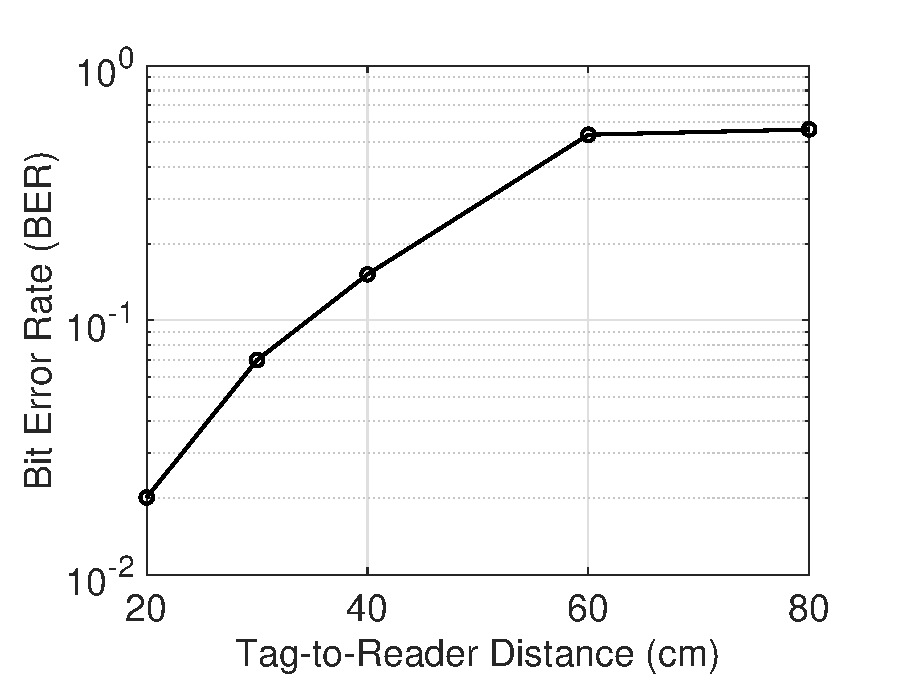
\includegraphics[width=0.8\columnwidth]{Figures/Fig14.eps}
\caption{Measured Bit Error Rate (BER) versus the tag-to-reader distance. A  FM station $34$~Km away was used and  the communication bit rate was  $345$~bps.}
\label{fig:BER_ind}
\end{figure}
%
The  system was also tested indoors using the most  powerful FM station that was measured in the building. \cite{daskalakis2017ambient}. 
%
It corresponds to the  BBC $95.8$~MHz station which is located around $34.65$~Km away from experimental setup.
%
 The  radiated power of the FM station was $250$~KW 
and the power of the received FM signal next to the tag 
antenna, was measured with a spectrum analyser at $-40$~dBm.
%
The BER was measured for different tag-to-reader distances.
and the BER results are shown in Fig.~\ref{fig:BER_ind} for a fixed bit rate of  $345$ bps.

\begin{comment}
A link budget  was also calculated to estimate the received power of our signal \cite{griffin2009complete}. 
%
The FM backscatter system is similar to a bistatic radar setup where the FM station source and FM receiver are physically separated.
%

Referring to the geometry of Fig.~\ref{fig:chamber}
and assuming free space propagation between the emitter and the tag we can calculate the 
differential received power at the  SDR as \cite{ensworth2017ble}:
\begin{equation}
P_\text{SDR} = \frac{ \text{EIRP} \Delta\sigma G_\text{SDR}\lambda^2} {(4\pi)^3 D_\text{tag-SDR}^2 D_\text{FM-tag}^2}\\
\label{eq:t01}
\end{equation}
with $G_\text{SDR}$, $D_\text{tag-SDR}$,  the receiver antenna gain and tag-to-receiver distance respectively. $D_\text{FM-tag}$ is the distance from the FM station to the tag, and $\text{EIRP}$ is the effective isotropic radiated power of the FM station. 
%
The $P_\text{SDR}$  is proportional to the differential radar cross section (RCS) of the tag \cite{thomas2012quadrature, BleDimSah:j10,nikitin2007differential}:
%
\begin{equation}
\Delta\sigma = \frac{\lambda^2} {4\pi} G_\text{tag}^2 |\Gamma_\text{i}^*-\Gamma_\text{i+1}^*|^2\\
\label{eq:t01}
\end{equation} 
%
where $G_\text{tag}$ is the tag antenna gain and $\Gamma_i^*$ is the conjugate  reflection coefficient.
%
For our calculations we assumed,   the  frequency  of $95.8$~MHz, $G_\text{tag}=G_\text{SDR}=0.5$~dBi, $D_\text{tag-SDR}=0.8$~m and  $D_\text{FM-tag}=34.65$~km.  
%
Using the four reflection coefficients of Table~\ref{tab:gammas}, we estimated the three received power magnitudes as:  $-40.9$,  $-40.4$ and  $-41.2$~dBm.

\end{comment}

%
%The 4-PAM high order modulation is less efficient compared to the binary modulation referred in \cite{daskalakis2017ambient}.
% 
%With 4-PAM we need higher SNR to get the same BER that we would get with 2-PAM.
%
\begin{table}[t]	
\renewcommand{\arraystretch}{1.1}
\centering
\caption{Tag Power Consumption Characteristics}
\scalebox{1}
{
\begin{tabular}{c||c||c}
\hline
\hline
%\begin{tabular}[x]{@{}c@{}}MSE(Hz$^2$)\\pre-filt.\end{tabular} For forcing newline in cell
Operation Mode  &  $\mu$W & Bit rate (kbps) \\
\hline
\hline
Sleep: (no DAC, no ADC) &$1.08$ & 0\\
\hline
Active: $2$-ASK (no DAC, no ADC)&$6.48$ & $0.147$\\
\hline
Active: $2$-ASK (no DAC, ADC)&$396$&$0.147$\\
\hline
Active: $4$-PAM (DAC, no ADC)&$27$ & $0.345$\\
\hline
Active: $4$-PAM  (DAC, ADC)&$432$& $0.345$\\
\hline
Active: $4$-PAM (DAC, no ADC)&$283$ & $10.2$\\
\hline
Active: $4$-PAM (DAC, ADC)&$501$ & $10.2$\\

\hline
\hline
\end{tabular}
}
\label{tab:power}
\end{table}
%


	
\begin{table*}[t]	
\renewcommand{\arraystretch}{1}
\centering
\caption{High order Modulation Backscatter Designs}
\scalebox{1}
{
\begin{tabular}{c||c||c||c||c||c||c||c}
\hline
\hline
%\begin{tabular}[x]{@{}c@{}}MSE(Hz$^2$)\\pre-filt.\end{tabular} For forcing newline in cell
Work & Modulation & Backscatter Signal &  Power & Part & Bit rate & Energy/bit & Range (m)\\
\hline
This work & $4$-PAM & Ambient FM&$27~\mu$W (Measurement) & Tag+Modulator & $345$~bps & $78.2$~nJ/bit & $1$ \\
\hline
This work & $4$-PAM&  Ambient FM &$501~\mu$W (Measurement)& Tag+Modulator & $10.2$~Kbps& $27.7$~nJ/bit &- \\
\hline
\cite{thomas2012quadrature}&$4$-QAM &  UHF CW& $115$~nW+$6$mW (Measurement) & Tag+Modulator &$400$~kbps& $15$~nJ/bit & $2.92$\\
\hline
\cite{thomas201296}&$16$-QAM&  UHF CW& $1.49$~mW (Measurement) & Modulator &$96$~Mbps& $15.5$~pJ/bit & $1.24$\\
\hline
\cite{correia2017quadrature} &$16$-QAM&  UHF CW &$1$~mW (Measurement) & Modulator &$60$~Mbps &$6.7$~pJ/bit &- \\
\hline
\cite{shirane201513}&$32$-QAM& $5.8$ GHz CW & $113~\mu$W (Simulation) & Tag+Modulator & $2.5$~Mbps& $49.1$~pJ/bit &-\\
\hline
 \cite{qian2018iot}&$4$-PSK&  UHF TV & - & Tag+Modulator & $20$~kbps& -& $0.7$\\
\hline
\cite{correia2018dual}&$4$-QAM& Cellular \& Wi-Fi & $27$~nW (Simulation) & Modulator & $500$~kbps& $0.054$~pJ/bit &- \\
\hline
\cite{wang2017fm}&$4$-FSK&  Ambient FM& $11.07~\mu$W (Simulation) & Tag+Modulator & $3.2$~kbps& $3.46$~nJ/bit& $4.8$\\



\hline
\hline
\end{tabular}
}
\label{tab:comparison}
\end{table*}

%There is a clear trade-off between performance and  spectral efficiency. 
%
%Given a baseband channel with bandwidth $B$ and a PAM constellation, by increasing the  order of  modulation ($m=2$) we can  increase the spectral efficiency $R_b/B=2m$ bps/Hz  and we can transmit  with a higher bit rate $R_b$. 
%
%The performance of modulation is decreased thus given a fixed  BER value, the SNR that is necessary to achieve   must be increased with $m$.


For power consumtion comparison and validation purposes,  $2$-ASK binary modulation  with FM0 encoding \cite{daskalakis2017ambient} was designed on this proof-of-concept tag. 
%
The proposed MCU was used without the DAC thus binary modulation requires only a digital output pin in order to control the transistor.
%
For the $2$-ASK and using the clock of $32$~kHz, the minimum $T_\text{symbol}$ achieved was $3.4$~ms and it corresponds to  a bit rate of $147$~bps.
% 
Table~\ref{tab:power} presents the  average power consumption results for $2$-ASK and $4$-PAM in addition to corresponding bit rates.
%
In binary modulation the average power dissipation was measured  at $6.48~\mu$W when the ADC was off and $396~\mu$W when the ADC was activated. 
%
The ADC is used for sensing and it  is turned off exactly after  the data collection in order to reduce the average power consumption.
%
Using the high order modulation, the $4$-PAM was measured at $27~\mu$W with the ADC disabled and $432~\mu$W with ADC turned on.
%
The proposed tag was programmed in a higher bit rate of $10.2$~Kbps only for power measurements purpose  and the power consumption was measured at $501~\mu$W when the ADC was turned on and $501~\mu$W when the ADC was off. 
%
An increment of  power consumption of the tag plus the modulator (RF transistor) is observed  for $4$-PAM when is programmed  at a higher bit rate.
%
%The maximum power consumption of the modulator  can be estimated using the formula : 
%$ P_\text{dymamic} < (1/2)CF_\text{max}V_\text{DD}^2$
%According to the transistor data sheet\cite{ATF52189} the gate Leakage Current ($I_\text{leak}$)
%
%The switching  will depend only on the Cgs capacitance
%
There is also a trade-off between the
bit rate and the power  consumption across  the two
modulation schemes.
% 
The bit rate is almost duplicated  but the consumption is not, due to the non-linear behaviour of the DAC component.


\section{Discussion}
\label{Sec:Discussion}

The DC power consumption reported in this work compared
 with  all the similar referenced works so far, are summarized in  Table~\ref{tab:comparison}. 
 The table presents all the designs 
that include hardware implementation  and use only high order modulation over a CW/ambient signal in order to communicate.
%
Our tag has been measured at low bit rate using ambient FM signals for communication and ensure fair comparison with the other works.
%
As shown, this works represents the lowest power consumption ambient backscatter hardware prototype implementation with high order modulation, reported to date.
%
The energy per bit was calculated  at $78$~nJ/bit for $345$~bps  and $27.7$~nJ/bit for $10.2$~kbps 
including the  energy consumption of the  modulator (RF transistor). 
%
In \cite{thomas2012quadrature} the static DC power consumption of the modulator,
excluding the power consumption of the microcontroller, was  $115$~nW corresponding to a data rate of
$400$~kbps.
%
The tag was fixed at $2.92$~m away from the transmitter  antenna with effective isotropic radiated power (EIRP)  $+38.4$~dBm.
%
In their prototype tag, a MSP430 microcontroller  was consuming an additional  $3-6$~mW
when generating the  data. 
%
A CR2032 $3$~V lithium coin cell battery was used  as a power source for the device.
%
In \cite{thomas201296} the semi-passive device was using a CR2032 $3$~V coin cell battery for DC power  and it was capable of transmitting $96$~Mbps with the modulator consuming  $1.49$~mW ($15.5$~pJ/bit).
% 
Using a transmitter with $+23$ dBm EIRP 
the backscatter data link had a measured operating distance of $1.24$~m in a typical indoor environment.
%
The \cite{thomas2012quadrature, thomas201296} were utilizing $4$-QAM and $16$-QAM respectively on an UHF CW signal. 
%
In \cite{correia2017quadrature} the value of energy
spent in the $16$-QAM  modulator was $16.7$~pJ/bit  for a data rate of $60$~Mbps  and the average power consumption was estimated at $1$~mW. 
%
\cite{shirane201513} presents a $113~\mu$W
$32$-QAM transmitter employing the  backscattering technique for the transmitting part. 
%
In \cite{qian2018iot} a $4$-PSK hardware prototype link  was implemented using ambient signals.
%
Two tags can communicate with information rate of $20$~kbps over a distance of $0.7$~m.
%
An RF source was  setup to transmit the single tone at $539$~MHz with power $10$~dBm.
%
 In \cite{correia2018dual},  a system capable of modulating the ambient signals was designed  for two different ambient sources (cellular and Wi-Fi signals) with $4$-QAM high order modulation. 
% 
Considering a data rate
of $500$ kbps, the power consumption of the modulator was $27$~nW with $0.054$~pJ energy per bit.  
%
The designs of \cite{correia2017quadrature, correia2018dual} were tested  using a signal generator to generate the transmitter signals 
 and an arbitrary waveform generator  to generate the voltage levels at the gate of each transistor. 
%
A coupler was used to measure the reflected signal from the circuit, by a VNA.
%
%
Finally, in  \cite{wang2017fm}, the ambient signals  were  used for communication and for their tag, they  simulated an integrated circuit that backscatters audio signals, and showed that it consumes $11.07~\mu$W at $3.2$~kbps bit rate.
%
For testing their $4$-FSK modulator prototype, they used an arbitrary waveform generator.
%
A USRP transmitter was setup to broadcast  mono and stereo audio signals with power up to $-60$ dBm.
% 
For transmit power $-60$ dBm at $1.6$ and $3.2$ kbps, the BER was low at distances (tag-to-reader) as high as $4.8$~m.
%
Further, at $1.6$~kbps, the BERs were still low up to $0.9$~m and $1.82$~m at $-60$ and $-50$~dBm respectively.
%

An alternative solution for our RF front-end is the use of four lumped impedances instead of one transistor. 
%
For example, the modulator in \cite{thomas2012quadrature, qian2018iot} includes a $4$-to-$1$ Mux (a SP4T CMOS RF switch) to modulate the circuit impedance between $4$ impedance states. 
%
It can be thought of as an ``impedance DAC" that converts a 2-bit digital input to a specified modulating impedance. 
%
The multi-state RF switch based modulator is power efficient as the DAC solution, though it trades off the board area and the more complex implementation. 
%
In case of an IC implementation it is required  bigger die area because $4$ switched impedances are required to implement $4$-ary modulation.  
%
The solution of a simple impedance transistor and a DAC 
seems to be a promising solution with similar power consumption but reduced die area.



A future challenge for this  work is to employ communication measurements (BER) for the $2$-PAM using this tag and compare them with the existing  high order modulation results. 
%
%
Finally, a new  compact RF front-end  could be designed and optimized together with a coil FM antenna on the same substrate.
%
At the receiver part, we focus to transmit our useful signals to smartphones using FM backscatter
communication. 
%
The TV signals are an alternative solution for the ambient source due to their shorter wavelength which means small antennas. 
%
Since our application will take advantage on the fact that smartphones have FM receivers, the TV signals do not fulfil our requirements.

The tag that is proposed in this work is semi-passive
since it uses a super capacitor for power supply.
%
With the utilization of the bistatic topology and semi-passive tags that communicate with a low bit rate, it is possible to implement a wireless sensor network, comprising the proposed low-cost sensor/tags.
%
The application shown in Fig.~\ref{fig:consept}   require that multiple tags could be supported. 
%
In that scenario, multiple tags could communicate with only one reader using a time-division-multiple-access (TDMA) scheme. 
%
Each tag could be programmed to work in a duty cycle operation in order to minimize the average power consumption.
%
Each  tag will be  active  only for a desired minimum period of time (i.e. send two packets) and  in ``sleep" mode for most of the time where the power consumption  is only $1.08~\mu$W.
%
The receiver could sent a pure CW signal in order to wake up the nearby tags from the ``sleep"  mode.  
%
The tags could send their information in random intervals in order to avoid a possible signal collision. 


\section{Conclusion}
\label{Sec:Conclusion}
%
In this work, we designed and integrated an ultra-low-power sensor node/tag
with ambient FM backscatter and high order modulation capabilities.
%
The tag can read up to four sensors and modulate the information using $4$-PAM modulation instead of the binary $2$-PAM.
%
The transmitted bit rate is duplicated and the tag uses the ambient FM signals in order to send the data to a low-cost SDR reader.
%
A real time algorithm was implemented in order to read the reflected
signals and  communication  was demonstrated experimentally indoors.
%
The tag does not require batteries and was supplied with a small solar panel consuming only $27~\mu$W.
%
This high order modulation approach is the first demonstration of
backscatter $4$-PAM modulation on ambient FM signals.
%
It also paves the way for practical deployments for short range, ultra-low-power backscatter  sensors such as wearable body area-sensors.
%



\section*{Acknowledgment}
\normalsize 

S. Daskalakis, G. Goussetis and A. Georgiadis would like to thank LRF and ICON. The authors would like to thank all members of  Microwaves and Antenna Engineering Research Group, Heriot-Watt University, Edinburgh, Scotland, UK EH14 4AS for their help in various steps throughout this work. 

 
\bibliographystyle{IEEEtran}
\begin{thebibliography}{10}
\providecommand{\url}[1]{#1}
\csname url@samestyle\endcsname
\providecommand{\newblock}{\relax}
\providecommand{\bibinfo}[2]{#2}
\providecommand{\BIBentrySTDinterwordspacing}{\spaceskip=0pt\relax}
\providecommand{\BIBentryALTinterwordstretchfactor}{4}
\providecommand{\BIBentryALTinterwordspacing}{\spaceskip=\fontdimen2\font plus
\BIBentryALTinterwordstretchfactor\fontdimen3\font minus
  \fontdimen4\font\relax}
\providecommand{\BIBforeignlanguage}[2]{{%
\expandafter\ifx\csname l@#1\endcsname\relax
\typeout{** WARNING: IEEEtran.bst: No hyphenation pattern has been}%
\typeout{** loaded for the language `#1'. Using the pattern for}%
\typeout{** the default language instead.}%
\else
\language=\csname l@#1\endcsname
\fi
#2}}
\providecommand{\BIBdecl}{\relax}
\BIBdecl

\bibitem{EPCRFID}
\BIBentryALTinterwordspacing
\emph{Specification for {RFID} Air Interface Protocol for Communications at 860
  MHz-960 MHz, Version 2.0.1}, EPC Global Inc., 2015. [Online]. Available:
  \url{https://www.gs1.org/sites/default/files/docs/epc/Gen2_Protocol_Standard.pdf}
\BIBentrySTDinterwordspacing

\bibitem{daskalakis2014soil}
S.~N. Daskalakis, S.~D. Assimonis, E.~Kampianakis, and A.~Bletsas, ``Soil
  moisture wireless sensing with analog scatter radio, low power, ultra-low
  cost and extended communication ranges,'' in \emph{Proc. {IEEE} Sensors
  Conf.}, Valencia, {S}pain, Nov. 2014, pp. 122--125.

\bibitem{daskalakis2018uw}
S.~N. Daskalakis, G.~Goussetis, S.~D. Assimonis, M.~M. Tentzeris, and
  A.~Georgiadis, ``A u{W} backscatter-morse-leaf sensor for low-power
  agricultural wireless sensor networks,'' \emph{{IEEE} Sensors J.}, vol.~18,
  no.~19, pp. 7889--7898, Oct. 2018.

\bibitem{sample2008design}
A.~P. Sample, D.~J. Yeager, P.~S. Powledge, A.~V. Mamishev, and J.~R. Smith,
  ``Design of an {RFID}-based battery-free programmable sensing platform,''
  \emph{{IEEE} Trans. Instrum. Meas.}, vol.~57, no.~11, pp. 2608--2615, Jun.
  2008.

\bibitem{kampianakis2017dual}
E.~Kampianakis, A.~Sharma, J.~Arenas, and M.~S. Reynold, ``A dual-band wireless
  power transfer and backscatter communication approach for real-time
  neural/{EMG} data acquisition,'' \emph{{IEEE} J. of Radio Frequency
  Identification}, vol.~1, no.~1, pp. 100--107, Aug. 2017.

\bibitem{thomas2010qam}
S.~Thomas and M.~S. Reynolds, ``{QAM} backscatter for passive {UHF RFID}
  tags,'' in \emph{Proc. {IEEE} Int. Conf. on RFID}, Orlando, FL, USA, Apr.
  2010, pp. 210--214.

\bibitem{thomas2012quadrature}
S.~J. Thomas, E.~Wheeler, J.~Teizer, and M.~S. Reynolds, ``Quadrature amplitude
  modulated backscatter in passive and semipassive {UHF} {RFID} systems,''
  \emph{{IEEE} Trans. Microw. Theory Techn.}, vol.~60, no.~4, pp. 1175--1182,
  Apr. 2012.

\bibitem{kimionis2017millimeter}
J.~Kimionis, A.~Georgiadis, and M.~M. Tentzeris, ``Millimeter-wave backscatter:
  A quantum leap for gigabit communication, {RF} sensing, and wearables,'' in
  \emph{Proc. {IEEE} MTT-S Int. Microw. Symp. (IMS)}, Honolulu, HI, USA, Jun.
  2017, pp. 812--815.

\bibitem{thomas201296}
S.~J. Thomas and M.~S. Reynolds, ``A 96 {M}bit/sec, 15.5 p{J}/bit 16-{QAM}
  modulator for {UHF} backscatter communication,'' in \emph{Proc. {IEEE} Int.
  Conf. on RFID}, Orlando, FL, USA, Apr. 2012, pp. 185--190.

\bibitem{correia2017quadrature}
R.~Correia, A.~Boaventura, and N.~B. Carvalho, ``Quadrature amplitude
  backscatter modulator for passive wireless sensors in {I}o{T} applications,''
  \emph{{IEEE} Trans. Microw. Theory Techn.}, vol.~65, no.~4, pp. 1103--1110,
  Feb. 2017.

\bibitem{shirane201513}
A.~Shirane, H.~Tan, Y.~Fang, T.~Ibe, H.~Ito, N.~Ishihara, and K.~Masu, ``A 5.8
  {GH}z {RF}-powered transceiver with a 113 u{W} 32-{QAM} transmitter employing
  the {IF}-based quadrature backscattering technique,'' in \emph{Proc. {IEEE}
  Int. Solid-State Circuits Conf. (ISSCC)}, San {F}rancisco, CA, USA, 2015, pp.
  1--3.

\bibitem{boyer2014invited}
C.~Boyer and S.~Roy, ``Backscatter communication and {RFID}: Coding, energy,
  and {MIMO} analysis,'' \emph{{IEEE} Trans. on Commun.}, vol.~62, no.~3, pp.
  770--785, Mar. 2014.

\bibitem{liu2013ambient}
V.~Liu, A.~Parks, V.~Talla, S.~Gollakota, D.~Wetherall, and J.~R. Smith,
  ``Ambient backscatter: wireless communication out of thin air,'' \emph{ACM
  SIGCOMM Comput. Commun. Rev.}, vol.~43, no.~4, pp. 39--50, Oct. 2013.

\bibitem{van2017ambient}
N.~Van~Huynh, D.~T. Hoang, X.~Lu, D.~Niyato, P.~Wang, and D.~I. Kim, ``Ambient
  backscatter communications: A contemporary survey,'' \emph{arXiv preprint
  arXiv:1712.04804}, Dec. 2017.

\bibitem{qian2018iot}
J.~Qian, A.~N. Parks, J.~R. Smith, F.~Gao, and S.~Jin, ``{I}o{T} communications
  with {M-PSK} modulated ambient backscatter: Algorithm, analysis, and
  implementation,'' \emph{{IEEE} Internet of Things J.}, Jul. 2018.

\bibitem{correia2018dual}
R.~Correia and N.~B. Carvalho, ``Dual-band high order modulation ambient
  backscatter,'' in \emph{Proc. {IEEE} MTT-S Int. Microw. Symp. (IMS)},
  Philadelphia, Pennsylvania, USA, Jun. 2018, pp. 270--273.

\bibitem{wang2017fm}
A.~Wang, V.~Iyer, V.~Talla, J.~R. Smith, and S.~Gollakota, ``{FM} backscatter:
  Enabling connected cities and smart fabrics,'' in \emph{Proc. USENIX Symp. on
  Networked Sys. Design and Impl. (NSDI)}, Boston, MA, Mar. 2017, pp. 243--258.

\bibitem{daskalakis2017ambient}
S.~N. Daskalakis, J.~Kimionis, A.~Collado, G.~Goussetis, M.~M. Tentzeris, and
  A.~Georgiadis, ``Ambient backscatterers using {FM} broadcasting for low cost
  and low power wireless applications,'' \emph{{IEEE} Trans. Microw. Theory
  Techn.}, vol.~PP, no.~99, pp. 1--12, Nov. 2017.

\bibitem{daskalakisims2018}
S.~N. Daskalakis, R.~Correia, G.~Goussetis, M.~M. Tentzeris, N.~B. Carvalho,
  and A.~Georgiadis, ``Spectrally efficient 4-{PAM} ambient {FM} backscattering
  for wireless sensing and {RFID} applications,'' in \emph{Proc. {IEEE} MTT-S
  Int. Microw. Symp. (IMS)}, Philadelphia, Pennsylvania, USA, Jun. 2018.

\bibitem{PIC16LF1459}
\BIBentryALTinterwordspacing
\emph{{PIC16LF1459}, {USB} Microcontroller with Extreme Low-Power Technology,
  product manual}, {M}icrochip {T}echnology {I}nc., 2014. [Online]. Available:
  \url{http://www.microchip.com/downloads/en/DeviceDoc/40001639B.pdf}
\BIBentrySTDinterwordspacing

\bibitem{SP3-37}
\BIBentryALTinterwordspacing
\emph{{SP3-37} {F}lexible {S}olar {P}anel 3{V} @ 22mA, product manual},
  {P}owerFilm, 2009. [Online]. Available: \url{https://goo.gl/q5ECXh}
\BIBentrySTDinterwordspacing

\bibitem{XC6504}
\BIBentryALTinterwordspacing
\emph{{XC6504} Ultra Low Power Consumption Voltage Regulator, product manual},
  {U}orex {S}emiconductor, 2012. [Online]. Available:
  \url{https://www.torexsemi.com/file/xc6504/XC6504.pdf}
\BIBentrySTDinterwordspacing

\bibitem{assimonis2014efficient}
S.~D. Assimonis, S.~N. Daskalakis, and A.~Bletsas, ``Efficient {RF} harvesting
  for low-power input with low-cost lossy substrate rectenna grid,'' in
  \emph{Proc. {IEEE} Conf. on RFID Techn. and Appl. (RFID-TA)}, Tampere,
  {F}inland, Sep. 2014, pp. 1--6.

\bibitem{niotaki2014solar}
K.~Niotaki, A.~Collado, A.~Georgiadis, S.~Kim, and M.~M. Tentzeris,
  ``Solar/{E}lectromagnetic energy harvesting and wireless power
  transmission,'' \emph{Proc. {IEEE}}, vol. 102, no.~11, pp. 1712--1722, Nov.
  2014.

\bibitem{gu2018integrated}
X.~Gu, S.~Hemour, L.~Guo, and K.~Wu, ``Integrated cooperative ambient power
  harvester collecting ubiquitous radio frequency and kinetic energy,''
  \emph{{IEEE} Trans. Microw. Theory Techn.}, vol.~66, no.~9, pp. 4178--4190,
  Sep. 2018.

\bibitem{ATF52189}
\BIBentryALTinterwordspacing
\emph{{ATF-52189} {H}igh {L}inearity {M}ode {E}nhancement {P}seudomorphic {HEMT
  FET} {T}ransistor, product manual}, {B}roadcom, 2006. [Online]. Available:
  \url{https://www.broadcom.com/products/wireless/transistors/fet/atf-52189#}
\BIBentrySTDinterwordspacing

\bibitem{BleDimSah:j10}
A.~Bletsas, A.~G. Dimitriou, and J.~N. Sahalos, ``Improving backscatter radio
  tag efficiency,'' \emph{{IEEE} Trans. Microw. Theory Techn.}, vol.~58, no.~6,
  pp. 1502--1509, Jun. 2010.

\bibitem{johnson2011software}
C.~R. Johnson~Jr, W.~A. Sethares, and A.~G. Klein, \emph{Software receiver
  design: build your own digital communication system in five easy
  steps}.\hskip 1em plus 0.5em minus 0.4em\relax Cambridge Univ. Press, 2011.

\bibitem{proakis2008digital}
J.~G. Proakis and M.~Salehi, \emph{Digital Communications fifth edition,
  2007}.\hskip 1em plus 0.5em minus 0.4em\relax McGraw-Hill Companies, Inc.,
  New York, NY, 2008.

\bibitem{qian2017noncoherent}
J.~Qian, F.~Gao, G.~Wang, S.~Jin, and H.~Zhu, ``Noncoherent detections for
  ambient backscatter system,'' \emph{{IEEE} Trans. Wireless Commun.}, vol.~16,
  no.~3, pp. 1412--1422, Dec. 2017.

\bibitem{alevizos2016log}
P.~N. Alevizos, Y.~Fountzoulas, G.~N. Karystinos, and A.~Bletsas,
  ``Log-linear-complexity {GLRT}-optimal noncoherent sequence detection for
  orthogonal and {RFID}-oriented modulations,'' \emph{{IEEE} Trans. on
  Commun.}, vol.~64, no.~4, pp. 1600--1612, Apr. 2016.

\bibitem{NESDR}
\BIBentryALTinterwordspacing
\emph{{NESDR} {SMA}rt {B}undle-Premium {RTL-SDR}, product manual}, Noo{E}lec
  {I}nc., 2017. [Online]. Available:
  \url{http://www.nooelec.com/store/nesdr-smart.html}
\BIBentrySTDinterwordspacing

\bibitem{clarke2014maximizing}
B.~Clarke and K.~Kreitzer, ``Maximizing the dynamic range of software-defined
  radio,'' \emph{Analog Devices Technical Article MS-2735}, pp. 1--4, 2014.

\bibitem{bamiedakisMSc}
M.~Bamiedakis-Pananos, ``Synchronization and {D}etection for {G}en2 {RFID}
  {S}ignals,'' Master's thesis, School of Electrical and Computer Engineering,
  Technical University of Crete, Greece, 2015.

\end{thebibliography}

%%%%%%%%%%%%%%%%%%%%%%%%%%%%%%%%%%%%%%%%%%%%%
\begin{IEEEbiography}[{\includegraphics[width=1in,height=1.55in,clip,keepaspectratio]{Figures/Fig18.png}}]
{Spyridon Nektarios Daskalakis} (S'12) was born in Heraklion, Greece in 1991. He received with excellence his Engineering Diploma and the M.Sc. in Electrical and Computer Engineering from Technical University of Crete (TUC) in 2014 and 2016, respectively. He is currently working toward the PhD degree in School of Engineering and Physical Sciences from Heriot-Watt university, Edinburgh UK. 

His current research interests include low-power, low-cost wireless sensor networks and energy harvesting. Particularly he focuses on backscatter radio communication, batteryless sensors, low cost software-defined radio, environmental sensing and RF energy harvesting. 
He has received fellowship award by the Clinton Global Initiative University 2014 (USA), the Onassis Foundation (graduate studies 2015/16 scholarship), the Lloyds Register Foundation (LRF) and the International Consortium in Nanotechnology (ICON). He was a recipient for two short-term scientific mission grands from COST Action IC1301 WiPE in School of Electrical and Computer Engineering, Georgia Institute of Technology, Atlanta in 2016, and the Centre Tecnològic de Telecomunicacions de Catalunya, Barcelona in 2015. He has been a member of the IEEE Microwave Theory and Techniques Society, the IEEE Council on RFID and the IEEE Sensors Council.
\end{IEEEbiography}

\begin{IEEEbiography}[{\includegraphics[width=1in,height=1.55in,clip,keepaspectratio]{Figures/Fig19.png}}]
{Ricardo Correia} (GS'15) is  a PhD student in Electrical Engineering at the University of Aveiro. He obtained his M.Sc. degree in Electronics and Telecommunications Engineering from the University of Aveiro in 2009. He worked one year as an automation and electrical engineer and three years as a researcher in embedded systems and signal processing.
Currently, he is a researcher at Institute of Telecommunications - University of Aveiro and his research interests include wireless power transfer, energy harvesting, wireless passive sensors for space applications and low power communications.

Mr. Correia is a student member of IEEE, and a member of IEEE Microwave Theory and Techniques Society (MTT-S). He is also a reviewer for IET Microwaves, Antennas \& Propagation, Wireless Power Transfer journal and IEEE Transactions on Microwave Theory and Techniques. He was the recipient of the 2016 URSI/ANACOM Prize, awarded by URSI Portuguese section and Portuguese National Authority of Communications (ANACOM).
\end{IEEEbiography}
%%%%%%%%%%%%%%%%%%%%%%%%%%%%%%%%%%%%%%%%%%%%%%%%%%%%%%%%%
\begin{IEEEbiography}[{\includegraphics[width=0.95in,height=1.55in,clip,keepaspectratio]{Figures/Fig20.png}}]
{George Goussetis} (S'99-M'02-SM'12) received the Diploma degree in Electrical and Computer Engineering from the National Technical University of Athens, Greece, in 1998, and the Ph.D. degree from the University of Westminster, London, UK, in 2002. In 2002 he also graduated B.Sc. in physics (first class) from University College London (UCL), UK. 

In 1998, he joined the Space Engineering, Rome, Italy, as RF Engineer and in 1999 the Wireless Communications Research Group, University of Westminster, UK, as a Research Assistant. Between 2002 and 2006 he was a Senior Research Fellow at Loughborough University, UK. He was a Lecturer (Assistant Professor) with Heriot-Watt University, Edinburgh, UK between 2006 and 2009 and a Reader (Associate Professor) with Queen’s University Belfast, UK, between 2009 and 2013. In 2013 he joined Heriot-Watt as a Reader and was promoted to Professor in 2014, where he currently directs the Institute of Sensors Signals and Systems. He has authored or co-authored over 500 peer-reviewed papers five book chapters one book and four patents. His research interests are in the area of microwave and antenna components and subsystems. 

Dr. Goussetis has held a research fellowship from the Onassis foundation in 2001, a research fellowship from the UK Royal Academy of Engineering between 2006-2011 and European Marie-Curie experienced researcher fellowships in 2011-12 and again in 2014-17. He is the co-recipient of the 2011 European Space Agency young engineer of the year prize, the 2011 EuCAP best student paper prize, the 2012 EuCAP best antenna theory paper prize and the 2016 Bell Labs prize. He has served as Associate Editor to the IEEE Antennas and Wireless Propagation Letters.

\end{IEEEbiography}


%%%%%%%%%%%%%%%%%%%%%%%%%%%%%%%%%%%%%
\begin{IEEEbiography}[{\includegraphics[width=1in,height=1.55in,clip,keepaspectratio]{Figures/Fig21.jpg}}]
{Manos M. Tentzeris}  (S'89-M'98-SM'03-F'10) received the Diploma Degree in Electrical and Computer Engineering from the National Technical University of Athens (``Magna Cum Laude") in Greece and the M.S. and Ph.D. degrees in Electrical Engineering and Computer Science from the University of Michigan, Ann Arbor, MI and he is currently Ken Byers Professor in Flexible Electronics with School of ECE, Georgia Tech, Atlanta, GA

He has published more than 650 papers in refereed Journals and Conference Proceedings, 5 books and 25 book chapters. Dr. Tentzeris has helped develop academic programs in 3D/inkjet-printed RF electronics and modules, flexible electronics, origami and morphing electromagnetics, Highly Integrated/Multilayer Packaging for RF and Wireless Applications using ceramic and organic flexible materials, paper-based RFID's and sensors, wireless sensors and biosensors, wearable electronics, ``Green" electronics, energy harvesting and wireless power transfer, nanotechnology applications in RF, Microwave MEM's, SOP-integrated (UWB, multiband, mmW, conformal) antennas and heads the ATHENA research group (20 researchers). He has served as the Head of the GT-ECE Electromagnetics Technical Interest Group, as the Georgia Electronic Design Center Associate Director for RFID/Sensors research and as the Georgia Tech NSF-Packaging Research Center Associate Director for RF Research and the RF Alliance Leader.  He was the recipient/co-recipient of the 2017 Georgia Tech Outstanding Achievement in Research Program Development Award, 2016 Bell Labs Award Competition 3rd Prize, the 2015  IET Microwaves, Antennas and Propagation Premium Award, the 2014 Georgia Tech ECE Distinguished Faculty Achievement Award, the 2014 IEEE RFID-TA Best Student Paper Award, the 2013 IET Microwaves, Antennas and Propagation Premium Award, the 2012 FiDiPro Award in Finland, the iCMG Architecture Award of Excellence, the 2010 IEEE Antennas and Propagation Society Piergiorgio L. E. Uslenghi Letters Prize Paper Award, the 2011 International Workshop on Structural Health Monitoring Best Student Paper Award, the 2010 Georgia Tech Senior Faculty Outstanding Undergraduate Research Mentor Award,  the 2009 IEEE Transactions on Components and Packaging Technologies Best Paper Award, the 2009 E.T.S. Walton Award from the Irish Science Foundation, the 2007 IEEE APS Symposium Best Student Paper Award, the 2007 IEEE IMS Third Best Student Paper Award, the 2007 ISAP 2007 Poster Presentation Award, the 2006 IEEE MTT Outstanding Young Engineer Award, the 2006 Asian-Pacific Microwave Conference Award, the 2004 IEEE Transactions on Advanced Packaging Commendable Paper Award, the 2003 NASA Godfrey ``Art" Anzic Collaborative Distinguished Publication Award, the 2003 IBC International Educator of the Year Award, the 2003 IEEE CPMT Outstanding Young Engineer Award, the 2002 International Conference on Microwave and Millimeter-Wave Technology Best Paper Award (Beijing, CHINA), the 2002 Georgia Tech-ECE Outstanding Junior Faculty Award, the 2001 ACES Conference Best Paper Award and the 2000 NSF CAREER Award and the 1997 Best Paper Award of the International Hybrid Microelectronics and Packaging Society. He was the TPC Chair for IEEE IMS 2008 Symposium and the Chair of the 2005 IEEE CEM-TD Workshop and he is the Vice-Chair of the RF Technical Committee (TC16) of the IEEE CPMT Society. He is the founder and chair of the RFID Technical Committee (TC24) of the IEEE MTT Society and the Secretary/Treasurer of the IEEE C-RFID. 

He is the Associate Editor of IEEE Transactions on Microwave Theory and Techniques, IEEE Transactions on Advanced Packaging and International Journal on Antennas and Propagation. 
Dr. Tentzeris was a Visiting Professor with the Technical University of Munich, Germany for the summer of 2002, a Visiting Professor with GTRI-Ireland in Athlone, Ireland for the summer of 2009 and a Visiting Professor with LAAS-CNRS in Toulouse, France for the summer of 2010. He has given more than 100 invited talks to various universities and companies all over the world. He is a Fellow of IEEE, a member of URSI-Commission D, a member of MTT-15 committee, an Associate Member of EuMA, a Fellow of the Electromagnetic Academy and a member of the Technical Chamber of Greece. Prof. Tentzeris served as one of the IEEE MTT-S Distinguished Microwave Lecturers from 2010-2012 and he is one of the IEEE CRFID Distinguished Lecturers.
\end{IEEEbiography}

%%%%%%%%%%%%%%%%%%%%%%%%%%%%%%%%%%%%%

\begin{IEEEbiography}[{\includegraphics[width=1in,height=1.55in,clip,keepaspectratio]{Figures/Fig22.png}}]
{Nuno Borges Carvalho} (S'97-M'00-SM'05-F'15)
was born in Luanda, Angola, in 1972. He received the Diploma and Doctoral degrees in electronics and telecommunications engineering from the University of Aveiro, Aveiro, Portugal, in 1995 and 2000, respectively.

He is currently a Full Professor and a Senior Research Scientist with the Institute of Telecommunications, University of Aveiro and an IEEE Fellow. He coauthored Intermodulation in Microwave and Wireless Circuits (Artech House, 2003), Microwave and Wireless Measurement Techniques (Cambridge University Press, 2013) and White Space Communication Technologies (Cambridge University Press, 2014). He has been a reviewer and author of over 200 papers in magazines and conferences. He is the Editor in Chief of the Cambridge Wireless Power Transfer Journal, an associate editor of the IEEE Microwave Magazine and former associate editor of the IEEE Transactions on Microwave Theory and Techniques and IET Microwaves Antennas and Propagation Journal.

He is the co-inventor of six patents. His main research interests include software-defined radio front-ends, wireless power transmission, nonlinear distortion analysis in microwave/wireless circuits and systems, and measurement of nonlinear phenomena. He has recently been involved in the design of dedicated radios and systems for newly emerging wireless technologies.
Dr. Borges Carvalho is a member of the IEEE MTT ADCOM, the chair of the IEEE MTT-20 Technical Committee and the past-chair of the IEEE Portuguese Section and MTT-11 and also belong to the technical committees, MTT-24 and MTT-26. He is also the vice-chair of the URSI Commission A (Metrology Group). He was the recipient of the 1995 University of Aveiro and the Portuguese Engineering Association Prize for the best 1995 student at the University of Aveiro, the 1998 Student Paper Competition (Third Place) of the IEEE Microwave Theory and Techniques Society (IEEE MTT-S) International Microwave Symposium (IMS), and the 2000 IEE Measurement Prize.
He is a Distinguished Microwave Lecturer for the IEEE Microwave Theory and Techniques Society.

\end{IEEEbiography}

%\vspace*{-2\baselineskip}
%%%%%%%%%%%%%%%%%%%%%%%%%%%%%%%%%%%%%

\begin{IEEEbiography}[{\includegraphics[width=1in,height=1.55in,clip,keepaspectratio]{Figures/Fig23.jpg}}]
{Apostolos Georgiadis} (S'94-M'02-SM'08) was
born in Thessaloniki, Greece. He received the B.S.
degree in physics and M.S. degree in telecommunications
from the Aristotle University of Thessaloniki,
Thessaloniki, Greece, in 1993 and 1996,
respectively, and the Ph.D. degree in electrical
engineering from the University of Massachusetts,
Amherst, MA, USA, in 2002.

In 2002, he joined Global Communications
Devices, North Andover, MA, USA, as a Systems
Engineer where he involved in CMOS transceivers
for wireless network applications. In 2003, he joined Bermai Inc., Minnetonka,
MN, USA, as an RF/Analog Systems Architect. In 2005, he joined the
University of Cantabria, Santander, Spain, as a Juan de la Cierva Fellow
Researcher. In 2006, he was a consultant for Bitwave Semiconductor, Lowell,
MA, USA. He collaborated with ACORDE S.A., Santander, Spain, where
he was involved in the design of integrated CMOS VCOs for ultra-wideband
applications. In 2007, he joined the Technological Telecommunications Center
of Catalonia (CTTC), Spain, as a Senior Researcher of communications
subsystems. From 2013 to 2016, he was a Group Leader with the Microwave
Systems and Nanotechnology Department, CTTC. In 2016, he joined Heriot-Watt University, Edinburgh, U.K., as an Associate Professor. He has authored
more than 180 papers in peer-reviewed journals and international conferences.
His current research interests include energy harvesting and wireless power
transmission, RFID technology, active antennas and phased-array antennas,
inkjet and 3-D printed electronics, millimeter-wave systems.

Dr. Georgiadis was a recipient of the Fulbright Scholarship for graduate studies at the University of Massachusetts, in 1996. He was the General Chair of the 2011 IEEE RFID-TA Conference and the General Co-Chair of the 2011 IEEE MTT-S IMWS on Millimeter Wave Integration Technologies. He is an EU Marie Curie Global Fellow. He is member of the IEEE MTT-S TC-24 RFID Technologies (past Chair) and a member of the IEEE MTT-S TC-26 Wireless Energy Transfer and Conversion. He was an Associate Editor of the IET Microwaves Antennas and Propagation journal, IEEE MICROWAVE AND WIRELESS COMPONENTS LETTERS, and the IEEE RADIO FREQUENCY IDENTIFICATION (RFID) VIRTUAL JOURNAL. He serves as an Associate Editor for the IEEE JOURNAL OF RFID and is the Founder and the Editor-in-Chief of the Wireless Power Transfer Journal of Cambridge University Press. He is the Chair of the URSI Commission D, Electronics, and Photonics, and an AdCom member of the IEEE Council on RFID serving as the Vice President of conferences. He is a Distinguished Lecturer of the IEEE Council on RFID. In 2016, his proposal for Inkjet/3-D printed millimeter-wave systems received the Bell Labs Prize, third place among more than 250 proposals recognizing ideas that ``change the game" in the field of information and communications technologies.
\end{IEEEbiography}
% that's all folks
\end{document}
